\documentclass[conference]{IEEEtran}
\IEEEoverridecommandlockouts
% The preceding line is only needed to identify funding in the first footnote. If that is unneeded, please comment it out.
\usepackage{cite}
\usepackage{amsmath,amssymb,amsfonts}
\usepackage{algorithmic}
\usepackage{graphicx}
\usepackage{textcomp}
\usepackage{xcolor}
\usepackage{listings}
\def\BibTeX{{\rm B\kern-.05em{\sc i\kern-.025em b}\kern-.08em
    T\kern-.1667em\lower.7ex\hbox{E}\kern-.125emX}}
\begin{document}

\title{RFID Sicherheit}


\author{\IEEEauthorblockN{Julian Hoever}
\IEEEauthorblockA{\textit{Verteilte Systeme} \\
\textit{Universität Duisburg-Essen}\\
Duisburg, Deutschland\\
julian.hoever@stud.uni-due.de}
}

\maketitle

\begin{abstract}
Die folgende Arbeit behandelt das Thema der RFID Sicherheit im Bezug auf Sicherheitslücken, Schutzmaßnahmen und Privatsphäre. Es werden einige mögliche Schwachstellen der RFID/NFC Technik aufgezeigt und Angriffstechniken vorgestellt, welche die zuvor aufgeführten Schwachstellen ausnutzen. Dabei wird darauf eingegangen, in welchen realen Szenarien diese Angriffe eine Bedrohung darstellen, wie zum Beispiel beim kontaktlosen Bezahlen oder der Diebstahlsicherung von Waren. Anschließend werden einige Schutzmaßnahmen skizziert, welche die zuvor genannten Angriffstechniken abmildern oder verhindern können und es wird diskutiert, wie durchführbar die genannten Angriffstechniken in der realen Welt sind. Dies hilft dabei abzuschätzen, wie relevant die Bedrohung ist, die von der RFID Technik in diesen Bereichen ausgeht. Abschließend wird noch der Aspekt der Einschränkung der Privatsphäre durch RFID Chips, besonders in Ausweisen aber auch in Produkten zur Diebstahlsicherung, besprochen und eingeordnet.
\end{abstract}

\section{Einleitung}
Die kontaktlose RFID Technik gehört bei vielen Menschen mittlerweile zum Alltag. Sie wird genutzt um kontaktlos Einkäufe zu bezahlen, auf der Arbeit mittels RFID Transponders die Eingangstür zu öffnen und bei einer Stempeluhr Arbeitszeiten zu dokumentieren. Die Einsatzbereiche der RFID Technik sind mittlerweile vielfältig. Eine weitere häufige Anwendung ist das Identifizieren von Gegenständen, zum Beispiel bei der Diebstahlsicherung von Waren oder der Verfolgung von Frachten. Durch die kontaktlosen Anwendungsbereiche bietet diese Technik einen erhöhten Komfort. Dafür wird häufig der Preis eines signifikant verringerten Sicherheitsniveaus oder eine Einschränkung der Privatsphäre gezahlt. Um eine Einschränkung der Sicherheit und Privatsphäre zu verhindern, müssen durch geeignete Schutzmaßnahmen Systeme die auf RFID beruhen abgesichert werden und dabei auch, falls erforderlich, Maßnahmen zu Schutz der Privatsphäre getroffen werden.

Aus diesem Grund wird in dieser Arbeit dargestellt, was die Probleme und möglichen Angriffsszenarien der RFID/NFC Technik sind. Dabei werden ausschließlich die passive RFID Transponder behandelt, da diese durch den einfachen Aufbau und das Fehlen einer eigenen Stromversorgung sehr weit verbreitet sind.

Zu Beginn wird dazu in Abschnitt 2 auf die Grundlagen der RFID/NFC Technik eingegangen. Anschließend beschreibt Abschnitt 3 was RFID/NFC konzeptionell für Schwachstellen besitzt. Darauf aufbauend wird dann in Abschnitt 4 erläutert was sich für mögliche Angriffe, auf die Sicherheit des Systems und die Privatsphäre der Nutzer, aus den in Abschnitt 3 genannten Schwachstellen ergeben. In Abschnitt 5 werden mögliche Sicherheitsmaßnahmen skizziert, welche Angriffe auf diese Technik erschweren und in Abschnitt 6 wird diskutiert wie durchführbar die vorgestellten Angriffe auf RFID Systeme in der Praxis überhaupt sind.


\section{Grundlagen}

\subsection{RFID Technik}
Radio Frequency Identification (RFID) ist eine Technik um kontaktlos Daten mittels eines Lesegerätes (Transceiver) aus einem Transponder auszulesen. Transponder gibt es in vielen verschiedenen Formen und Größen, je nach Anwendungsbereich. Grundlegend funktionieren alle Transponder aber recht ähnlich. Transponder bestehen in der Regel aus einer Antenne, in Form einer Spule, Schaltkreisen zum Senden/Empfangen und einem Speicher. Die Kommunikation erfolgt dann wie in Fig. \ref{fig1} dargestellt.

\begin{figure}[htbp]
\centerline{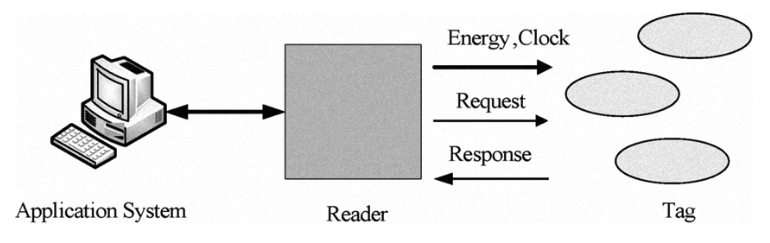
\includegraphics[width=0.5\textwidth]{img/kommunikation.png}}
\caption{Kommunikation zwischen Lesegerät (Reader) und Transponder \cite{b1}}
\label{fig1}
\end{figure}

Das Lesegerät (Reader) induziert über die spulenförmig angeordnete Antenne des Transponders, eine Spannung und Taktfrequenz, welche den Transponder mit dem nötigen Strom versorgt damit eine Kommunikation zwischen Lesegerät und Transponder stattfinden kann. Anschließend sendet das Lesegerät eine Anfrage an den Transponder, woraufhin ihm der Transponder seine Daten die er enthält übermittelt.

Bei den RFID Transpondern wird unterschieden zwischen passiven und aktiven Transpondern.
\begin{itemize}
\item Passive Transponder besitzen keine eigene Spannungsquelle und erreichen dadurch lediglich eine Reichweite von weniger als 4 Metern \cite{b1}.
\item Aktive Transponder hingegen besitzen zusätzlich noch eine eingebaute Spannungsquelle, meist in Form einer Batterie. Dadurch sind Reichweiten von über 100 Metern möglich \cite{b1}.
\end{itemize}
Wie bereits in der Einleitung angemerkt fokussiert sich diese Arbeit ausschließlich auf die passiven Transponder, da diese in im alltäglichen Leben, im Gegensatz zu den aktiven Transpondern, von größerer Bedeutung sind.

\subsection{NFC Technik}
NFC steht für Near Field Communication und ist ein Standard der der mit einer Frequenz von 13.56 MHz und einer Übertragungsgeschwindigkeit von 424 KBit/s arbeitet \cite{b2}. Dieser Standard ist für Datenübertragungen von bis zu 10 cm ausgelegt und setzt technisch direkt auf der RFID Technik auf \cite{b2}. Dies ermöglicht mittels eines NFC Lesegeräts, beispielsweise Smartphones, sogar RFID Transponder auszulesen. Zum Lesen und Schreiben wird auch hier ebenfalls mit einer spulenförmigen Antenne gearbeitet.

NFC kann in 3 Betriebsmodi betrieben werden \cite{b2}:

\begin{itemize}
\item Peer-to-Peer Modus
\item Lese-Schreib Modus
\item Kartenemulationsmodus
\end{itemize}

Bei dem Peer-to-Peer Modus findet zwischen beiden Geräten ein bidirektionaler Datenaustausch statt. Ein Beispiel dafür ist der Datenaustausch zwischen zwei Smartphones per NFC. Dabei agieren beide Smartphones als Sender und Empfänger.

Bei dem Lese-Schreib Modus fungiert das aktive Gerät als Lesegerät und das passive Gerät ist hierbei ein kompatibler passiver RFID Transponder zum Beispiel in einem Aufkleber oder einer Karte mit eingebautem RFID Transponder. Es ist in diesem Modus aber auch möglich, dass das aktive Gerät einen RFID Transponder, welcher noch nie beschrieben wurde, beschreibt.

Bei dem Kartenemulationsmodus simuliert das NFC Gerät einen passiven RFID Transponder was bedeutet, das dieses Gerät keinerlei Berechnungen durchführt und lediglich die festgelegten Daten an ein anfragendes Lesegerät übermittelt. Dies findet zum Beispiel beim kontaktlosen Bezahlen mittels Smartphone Anwendung.


\section{Schwachstellen}
Die RFID und NFC Technik besitzt vielerlei Schwachstellen und diese sind zum Großteil sowohl auf RFID als auch auf NFC anzuwenden. Der wichtigste Unterschied zwischen RFID und NFC ist die Reichweite auf denen diese Technik operiert. Bei NFC muss der Angriff viel näher am Lesegerät stattfinden als bei RFID, da mit passiven RFID Transpondern Reichweiten von bis zu 4 Metern erreicht werden können. Im folgenden werden einige mögliche Schwachstellen beider Techniken aufgelistet.

\subsection{Authentifikation}
Wie bereits in dem Abschnitt mit den Grundlagen der RFID Technik beschrieben, übermittelt ein RFID Transponder im wesentlichen seinen gesamten Speicherinhalt an ein anfragendes Lesegerät. Das bedeutet, dass keinerlei Authentifikation auf Seiten des Transponders stattfindet und damit jedes Lesegerät was auf der Frequenz des Transponders agiert den Transponder lesen kann, wodurch möglicherweise Daten in falsche Hände gelangen können. Jedoch gibt es seit einiger Zeit Transponder, welche eine Authentifikation durchführen bevor Daten übermittelt werden.

\subsection{Lesegerät kennt Daten nicht}
Ein weiteres Problem ist, dass das Lesegerät, welches Daten von einem Transponder anfragt, nicht weiß was für Daten es von dem Transponder erhält. Diese Daten müssen aber trotzdem verarbeitet werden. Dies kann ohne Sicherheitsvorkehrungen dazu führen, dass verarbeitende Prozesse oder Datenbanken, welche diese Daten speichern sollen, Schaden nehmen können.

\subsection{Lesegerät muss Transponder lesen}
Ein RFID/NFC Lesegerät muss, wenn ein Transponder in seine Nähe kommt, diesen Transponder auch lesen. Ohne den Transponder zu lesen, kann das Lesegerät nicht entscheiden ob dieser Transponder wichtig ist oder nicht. Damit besteht von außen die Möglichkeit Reaktionen des Lesegerätes herbeizuführen \cite{b3}. Dies stellt ebenfalls ein Problem dar und lässt sich wie im nächsten Kapitel genauer erläutert ausnutzen.

\subsection{Eindeutige Identifikation}
Des Weiteren lässt sich sowohl der Speicherinhalt als auch die eindeutige Identifikationsnummer des Transponders dazu verwenden diesen zu identifizieren. Dies ist in vielen Situationen vermutlich gewünscht, kann aber auch ein Sicherheitsrisiko darstellen.

\subsection{Energieversorgung}
Damit ein passiver RFID Transponder funktionieren kann muss durch das Lesegerät eine Spannung induziert werden, welche dafür sorgt, dass der Transponder Daten versenden kann. Wird der RFID Transponder zum Beispiel durch einen Faradayschen Käfig abgeschirmt, wird der RFID Transponder nicht mit Energie versorgt und das Lesegerät bekommt keine Daten von dem RFID Transponder übermittelt.

\subsection{Übertragung}
Ursprünglich ist RFID mit dem Standard ISO/IEC 18000 so standardisiert worden, dass die Übertragung zwischen Lesegerät und Transponder im Klartext geschieht. Dies sorgt dafür, dass die Übertragung abgehört werden kann.

\section{Angriffe auf Sicherheit und Privatsphäre}
Mit den im vorherigem Abschnitt beschriebenen Schwachstellen lassen sich mögliche Angriffsszenarien beschreiben welche die Sicherheit eines Systems ohne entsprechende Gegenmaßnahmen gefährden würden.

\subsection{Kopieren von Transpondern}
Bei der Verwendung von Transpondern ohne Authentifikation lässt sich der Transponder ohne weiteres mit einem kompatiblen Lesegerät auslesen. Die ausgelesenen Daten können anschließend dazu verwendet werden einen neuen uninitialisierten Transponder zu beschreiben um dadurch eine Kopie des ursprünglich gelesenen Transponders zu erhalten. Diese Kopie kann dann den gleichen Zweck erfüllen wie das Original. Angenommen der Originaltransponder wurde dazu verwendet eine Haustüre zu öffnen. Das bedeutet, dass es durch ein kurzes Auslesen des Originaltransponders möglich ist einen zweiten Hausschlüssel zu erzeugen. 

Diese Kopiervorgänge können innerhalb weniger Sekunden geschehen und brauchen nur einen flüchtigen Kontakt mit dem Originaltransponder. Dies kann zum Problem werden, wenn beispielsweise ein RFID Transponder an einem Schlüsselbund oder eine Karte in einer Brieftasche kurz aus den Augen gelassen wird. In der Zeit könnte ein Angreifer, ohne Aufmerksamkeit zu erregen, die Daten der jeweiligen Transponder kopiert haben.

\subsection{Kom­pro­mit­tie­ren des Lesegerätes}
Die Möglichkeit einfach einen RFID/NFC Transponder auszulesen stellt nicht nur ein Problem für die Sicherheit der Daten auf dem Transponder da. Durch das einfache Auslesen kann auch die Sicherheit des Lesegerätes und der darunter liegenden Softwareinfrastruktur entstehen. Dieses Problem entsteht dadurch, dass ein Lesegerät jeden Transponder liest, welcher sich in Reichweite ist. Befindet sich unter diesen Transpondern ein Transponder welcher Schadcode als Daten enthält, wird das Lesegerät, beispielsweise ein Smartphone oder eine Türsteuerung, dessen Daten ebenfalls lesen und verarbeiten. Wird auf Seiten des Lesegerätes nun nicht dafür gesorgt, dass Schadcode unschädlich gemacht wird, kommt dieser Schadcode ungehindert in tiefere Systembereiche.
Durch die verhältnismäßig kleine Speichergröße eines RFID Transponders von Bytes bis wenigen Kilobytes, beispielsweise 4 kB bei der MIFARE Classic EV1 4K \cite{b4}, ist die Größe des Schadcodes begrenzt, reicht aber aus um Schaden anzurichten \cite{b5}. Bei dem Schadcode kann es sich beispielsweise um SQL Injections handeln. Ein Beispielszenario wäre, dass ein Transponder mit einem schädlichen SQL Statement wie
\begin{lstlisting}
"; DROP TABLE <tabellenname>
\end{lstlisting}
\cite{b5} präpariert worden ist und dieser dann in die Nähe eines Lesegerätes gebracht wird. Das Lesegerät würde dann die Daten lesen und möglicherweise versuchen diese Daten in eine Datenbank zu schreiben. Das würde in der Datenbank dafür sorgen, dass die Tabelle mit dem in der SQL Injection angegebenen Tabellennamen gelöscht wird. Durch den Datenverlust entstehen in der Regel schwere Schäden auf Seiten des Lesegerätes und der dahinterstehen Softwareinfrastruktur.

\subsection{Erweitern von NFC zu Bluetooth}
Ein ähnliches Problem, was aber speziell NFC betrifft, ist die Koppelung von Bluetooth Verbindungen mittels NFC oder das Teilen von größeren Datenmengen eingeleitet über NFC. Dieses Angriffsszenario betrifft hauptsächlich Smartphones. Smartphones mit NFC besitzen oft die Möglichkeit über NFC Bluetooth Verbindungen herzustellen oder Daten zu teilen indem lediglich das Smartphone in die Nähe des anderen Gerätes gebracht wird. Beim Teilen von größeren Datenmengen über NFC wird auch häufig NFC nur zum Koppeln einer Bluetooth Verbindung genutzt und der eigentliche Datentransfer läuft anschließend über diese Bluetooth Verbindung \cite{b6}. Das Problem dabei ist, dass so die Kurzstreckenverbindung über NFC erweitert wurde auf eine Bluetooth Verbindung mit einer deutlich erhöhten Reichweite und einer schnelleren Übertragungsrate \cite{b6}. Diese Verbindung kann anschließend dafür genutzt werden aus größerer Entfernung Schadcode auf das Zielgerät zu schleusen.

\subsection{Tracking durch Transponder IDs}
Ein weiteres Problem ist die eindeutige Identifikationsnummer eines RFID Gerätes. Jedes RFID Gerät besitzt eine eindeutige Identifikationsnummer welche benötigt wird um Kollisionen bei der Übertragung zu verhindern \cite{b3}. Diese Identifikationsnummer bestimmt jeden Transponder und jedes RFID Gerät (und damit auch NFC Gerät) eindeutig und ermöglicht ein Tracking dieser Geräte. Dadurch kann massiv die Privatsphäre von Personen beeinträchtigt werden. Ein Szenario in dem diese Technik ausgenutzt werden könnte ist beispielsweise ein Unternehmen, in dem jeder Mitarbeiter RFID Transponder zum Zeitstempeln an Stempeluhren, Bezahlen in der Mensa und/oder zur Zugangskontrolle besitzt. Das Unternehmen könnte in dem Betrieb an vielen verschiedenen Stellen RFID Lesegeräte installieren. Diese Lesegeräte würden die Identifikationsnummer jedes RFID Transponders lesen, welcher in seine Reichweite kommt. Die Identifikationsnummer lassen sich dann Mitarbeitern zuordnen. Dadurch ist es möglich unbemerkt sämtliche Bewegungen der Mitarbeiter im Gebäude zu verfolgen. Diese Bewegungsprofile könnten anschließend dazu genutzt werden deren Arbeitszeit zu überwachen oder personelle Entscheidungen zu treffen.

Diese Art des Trackings wäre beispielsweise auch beim Einkaufen ein Problem. Geschäfte könnten an diversen Stellen im Laden RFID Lesegeräte platzieren und die Produkte mit RFID Transpondern zur Diebstahlsicherung ausstatten. Nimmt nun ein Kunde ein Produkt, und bewegt sich anschließend durch das Geschäft, registriert jedes Lesegerät, an dem der Kunde vorbei geht, die eindeutige Kennung des RFID Transponders. Dadurch wären die Geschäfte in der Lage das Konsumverhalten und die Laufwege der Kunden zu überwachen und so kann der gesamte Einkaufsprozess dieser Person genaustens nachverfolgt werden. Dies stellt ebenfalls eine erhebliche Gefährdung der Privatsphäre des Kunden dar.

\subsection{Denial of Service Angriffe}
Ebenfalls im Einzelhandel ist nicht nur das Tracking mittels RFID Transpondern ein Problem. Ein anderer wichtiger Angriff gegen RFID/NFC Technologie ist der Denial of Service. Beim Denial of Service Angriff geht es darum die Funktionsfähigkeit von RFID Transpondern oder Lesegeräten zu behindern, oder auch ganz funktionsunfähig zu machen. Diesen Punkt kann man aus zwei Perspektiven beleuchten. Entweder kann es darum gehen den Transponder funktionsunfähig zu machen oder es kann darum gehen ein Lesegerät funktionsunfähig zu machen. Beide Punkte werden im folgenden erläutert:

\subsubsection{Angriff auf Transponder}
Bei einem Denial of Service Angriff auf einen Transponder handelt es sich überwiegend um einen Angriff auf die Stromversorgung des Transponders. Mit einem solchen Angriff soll die Stromversorgung mittels Induktion verhindert werden. Dadurch kann der Transponder erst gar nicht aktiv werden und auch keine Daten austauschen. Eine Möglichkeit dies zu erreichen, ist es den Transponder durch einen so genannten Faradayschen Käfig abzuschirmen wie in Fig. \ref{fig2} dargestellt.

\begin{figure}[htbp]
\centerline{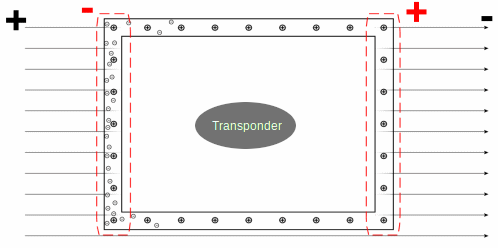
\includegraphics[width=0.5\textwidth]{img/kaefig.png}}
\caption{Transponder im Faradayschen Käfig \cite{b7}}
\label{fig2}
\end{figure}

Bei einem Faradayschen Käfig handelt es sich um eine vollständig geschlossene leitende Hülle. Wirkt ein elektrisches Feld auf diese Hülle ein sorgt der Faradaysche Käfig dafür, wie in Fig. \ref{fig2} dargestellt, dass dieses elektrische Feld nicht in das innere der Hülle vordringen kann. Das elektrische Feld ist in der Grafik dargestellt durch die waagerechten Linien und die Hülle als der rechteckige Kasten.

Für einen Transponder der in einen solchen Faradayschen Käfig gebracht wird, bedeutet dies, dass das vom Lesegerät erzeugte elektrische Feld zur Stromversorgung durch den Faradayschen Käfig abgehalten wird und nicht in das innere dieses Käfigs vordringen kann. Damit wird der, im inneren befindliche, Transponder nicht mit der nötigen Energie versorgt und es findet kein Datenaustausch zwischen Lesegerät und Transponder statt. Für das Lesegerät wirkt es so als sei der Transponder überhaupt nicht existent.

Ein daraus resultierendes Angriffsszenario wäre beispielsweise die Diebstahlsicherung von Waren im Einzelhandel. Bei der Diebstahlsicherung von beispielsweise Kleidung werden RFID Transponder dazu genutzt um einen Alarm auszulösen, wenn eine Person, ohne die Kleidung zu bezahlen, den Laden verlässt. Dieses unbefugte Verlassen des Ladens wird von RFID Lesegeräten am Ausgang des Ladens bemerkt, indem die RFID Transponder in den Kleidungsstücken beim Durchqueren der Lesegeräten erkannt werden. Wurde das Diebesgut aber vor Verlassen des Ladens in einen Faradayschen Käfig verstaut kann die Person den Laden verlassen ohne das die Lesegeräte am Ausgang Alarm schlagen. Dies kann unter Umständen für einen Einzelhändler hohe Verluste bedeuten.

\subsubsection{Angriff auf Lesegeräte}
Eine andere Möglichkeit einen Denial of Service Angriff durchzuführen ist, indem man versucht ein Lesegerät funktionsunfähig zu machen. Dabei wird ausgenutzt, dass ein aktives RFID/NFC Lesegerät jeden RFID/NFC Transponder in seiner Umgebung auslesen muss um zu entscheiden ob er wichtig für die Anwendung des Lesegerätes ist. Dieser Lesevorgang eines Transponders dauert einen kleine Zeitspanne, in der das Lesegerät nicht in der Lage ist andere Transponder zu lesen. Das bedeutet es gibt die Möglichkeit ein Lesegerät für einen kurzen Moment zu blockieren \cite{b3}.

Mit der Möglichkeit, das Lesegerät für einen kurzen Moment zu blockieren, lassen sich so genannte Jammer bauen. Ein Jammer ist ein Gegenstand auf dem eine große Anzahl an RFID Transpondern installiert ist. Gelangt so ein Jamming Gerät in die Reichweite eines Lesegerätes, kann dieses Lesegerät, durch die hohe Anzahl an gleichzeitigen Antworten, funktionsunfähig gemacht werden. Dies kann ebenfalls dafür genutzt werden um beispielsweise eine Diebstahlsicherung von Waren zu umgehen. Wenn man mit einer Ware mit RFID Transponder und dem Jammer durch die Lesegeräte am Ausgang des Geschäftes geht, sind diese Lesegeräte mit der Anzahl der RFID Transpondern überfordert und schlagen ebenfalls keinen Alarm.

\subsection{Abhören der Kommunikation}
Anstatt die Übertragung mittels Denial of Service Angriffe zu unterbinden, kann es auch von Interesse sein eine Übertragung abzuhören. Dies ist möglich, da die Kommunikation, nach ISO/IEC 18000, zwischen Lesegerät und Transponder grundlegend ohne Verschlüsselung stattfindet \cite{b3}. Der Grund für die meist fehlende Verschlüsselung bei der Kommunikation sind die Kosten und der Aufwand der damit verbunden ist. Jedoch ist die Technik dadurch verwundbar, was in einigen Situationen ein Problem darstellt.

Ein Angriff sieht wie folgt aus. Ein Angreifer begibt sich mit einem passenden Lesegerät in die Reichweite eines anderen Lesegerätes bei dem gerade eine Kommunikation zwischen Lesegerät und Transponder stattfindet. Der Angreifer kann über sein Lesegerät die Daten, die zwischen den legitimen Lesegerät und Transponder ausgetauscht werden, abhören und aufzeichnen. Wenn der Angreifer die Daten aufgezeichnet haben sollte, kann er diese Daten zu einem späteren Zeitpunkt dazu nutzen um diese selber an das Lesegerät zu versenden und damit eine Kommunikation mit dem echten Transponder vorzutäuschen \cite{b8}. 

Ein anderes Problem ist dass die gesammelten Informationen auch sensible personenbezogene Daten enthalten können, was eine Einschränkung der Privatsphäre bedeutet, wenn man diese Daten unverschlüsselt im Klartext überträgt.

\subsection{Man-In-The-Middle Angriff}
Eine Angriffstechnik die auf den zuvor beschriebenen Angriff aufbaut, ist der so genannte Man-In-The-Middle (MITM) Angriff. Bei dieser Angriffstechnik handelt es sich grundsätzlich um eine Kombination aus mehreren Angriffstechniken. Ein Man-In-The-Middle Angriff ist eine Kombination aus Abhören von Daten, Verändern von Daten und Weitersenden von Daten. Dabei beruht dieser Angriff stark auf der Schwachstelle, dass die Kommunikation zwischen RFID Lesegerät und Transponder unverschlüsselt stattfindet. In Fig. \ref{fig3} ist der Ablauf eines solchen Angriffs schematisch dargestellt.

\begin{figure}[htbp]
\centerline{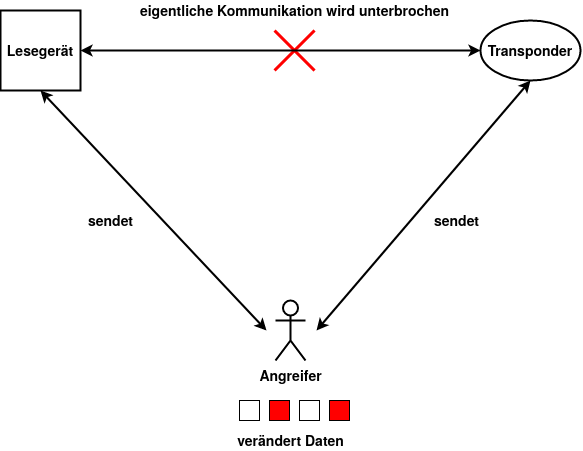
\includegraphics[width=0.5\textwidth]{img/MITM.png}}
\caption{Ablauf eines Man-In-The-Middle Angriffs}
\label{fig3}
\end{figure}

Für einen Man-In-The-Middle Angriff muss der Angreifer in der Lage sein die eigentliche Kommunikation zwischen Lesegerät und Transponder zu unterbrechen. Ist die Unterbrechung erfolgt muss nahtlos die die Kommunikation über den Angreifer umgeleitet werden, damit das Lesegerät diese Unterbrechung nicht bemerkt. Ist dieses Umleiten über den Angreifer erfolgreich durchgeführt worden, werden sämtliche Nachrichten die zwischen Lesegerät und Transponder ausgetauscht werden zuerst über den Angreifer weitergeleitet, der diese dann ebenfalls an den Transponder oder das Lesegerät weiterleitet. Dadurch ist der Angreifer in der Lage die gesamte Kommunikation zwischen Lesegerät und Transponder aufzuzeichnen ohne dass das Lesegerät diese Umleitung bemerkt.

Das Umleiten der Kommunikation ist in Fig. \ref{fig3} dargestellt als Doppelpfeil von Lesegerät zu Angreifer und Angreifer zu Transponder. Das rote Kreuz stellt die unterbrochene Kommunikation zwischen Lesegerät und Transponder dar.

Der Angreifer ist jedoch nicht nur in der Lage die Kommunikation zu belauschen. Da er sich unbemerkt zwischen der Kommunikation von Lesegerät und Transponder befindet und im Prinzip nur die Nachrichten weiterleitet die er erhält, ist er auch in der Lage die Nachrichten vor der Weiterleitung zu modifizieren oder blockieren. Der Transponder oder das Lesegerät ist dabei nicht in der Lage zu entscheiden ob die Pakete tatsächlich von dem legitimen Kommunikationspater oder von einem Angreifer kommen. Dadurch ist der Angreifer in der Lage falsche Informationen zu verteilen und den Datenaustausch zwischen Lesegerät und Transponder zu steuern wie es ihm beliebt.

Dies stellt ein erhebliches Problem im Bezug auf das Vertrauen und die Datenintegrität einer RFID/NFC Kommunikation dar.


\section{Sicherheitsmaßnahmen}
Nun wurden eine Reihe von Schwachstellen und Angriffstechniken beleuchtet, welche ernsthafte Probleme für die Sicherheit und Privatsphäre der Nutzer solcher Systeme darstellen. Viele der Schwachstellen wurden im Laufe der Jahre bereits behoben oder sind nur noch teilweise vorhanden. Aus diesem Grund werden als nächstes Sicherheitsmaßnahmen vorgestellt, die die schwere der vorgestellten Schwachstellen abmildern können, oder sogar ganz verhindern können. Dazu wird für jede Schwachstelle separat beleuchtet, wie dieses Problem abgesichert werden kann. Generell gilt für viele der hier vorgestellten Sicherheitsmaßnahmen, dass deren Sicherheit abhängt von 

\subsection{Authentifikation}
Wie bereits in dem vorherigen Abschnitt gesehen, stellt es ein großes Problem dar, wenn ein Transponder ohne Authentifizierung ausgelesen werden kann. Besonders wenn dieser Transponder für sicherheitskritische Systeme wie Türsteuerungen eingesetzt wird. Dies würde das einfache Auslesen und Kopieren eines Transponders ermöglichen. Um dieses Problem zu verhindern ist es notwendig eine Authentifizierung vor Datenaustausch mit dem Transponder durchzuführen. Dazu gibt es verschiedene Ansätze, die eine Authentifizierung zwischen Lesegerät und Transponder realisieren. Die Ansätze unterscheiden sich im wesentlichen an deren Sicherheit und Komplexität. Im folgenden wird der Ansatz der MIFARE Classic EV1 4k erläutert \cite{b4}.

\begin{figure}[htbp]
\centerline{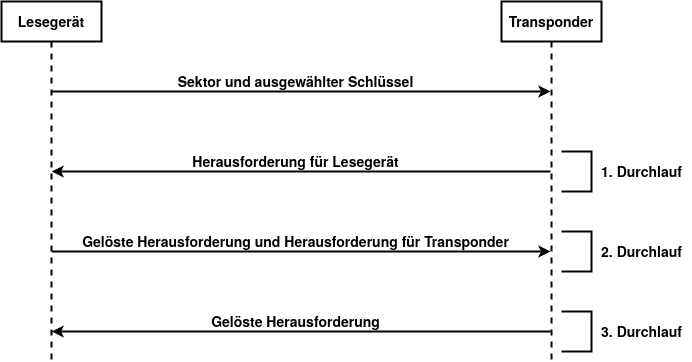
\includegraphics[width=0.5\textwidth]{img/three_pass.png}}
\caption{Drei-Phasen-Authentifikation der MIFARE Classic}
\label{fig4}
\end{figure}


\subsection{Lesegerät kennt Daten nicht}
[WORK IN PROGRESS]

\subsection{Lesegerät muss Transponder lesen}
[WORK IN PROGRESS]

\subsection{Eindeutige Identifikation}
[WORK IN PROGRESS]

\subsection{Energieversorgung}
[WORK IN PROGRESS]

\subsection{Übertragung}
[WORK IN PROGRESS]

\section{Durchführbarkeit der Angriffe}
[WORK IN PROGRESS]


\section{Fazit}
[WORK IN PROGRESS]


\begin{thebibliography}{00}
\bibitem{b1} Chih-Yung Chen, Chien-Ping Kuo and Fang-Yuan Chien, "An exploration of RFID information security and privacy," 2009 Joint Conferences on Pervasive Computing (JCPC), Tamsui, Taipei, 2009, pp. 65-70, doi: 10.1109/JCPC.2009.5420211.

\bibitem{b2} N. A. Chattha, "NFC — Vulnerabilities and defense," 2014 Conference on Information Assurance and Cyber Security (CIACS), Rawalpindi, 2014, pp. 35-38, doi: 10.1109/CIACS.2014.6861328.

\bibitem{b3} G. Madlmayr, J. Langer, C. Kantner and J. Scharinger, "NFC Devices: Security and Privacy," 2008 Third International Conference on Availability, Reliability and Security, Barcelona, 2008, pp. 642-647, doi: 10.1109/ARES.2008.105.

\bibitem{b4} NPX Semiconductors (32, November 2017) MIFARE Classic EV1 4K - Mainstream contactless smart card IC for fast and easy solution development. [Online]. Available: https://www.nxp.com/docs/en/data-sheet/MF1S70YYX\_V1.pdf.

\bibitem{b5} M. R. Rieback, B. Crispo and A. S. Tanenbaum, "Is your cat infected with a computer virus?," Fourth Annual IEEE International Conference on Pervasive Computing and Communications (PERCOM'06), Pisa, 2006, pp. 10 pp.-179, doi: 10.1109/PERCOM.2006.32.

\bibitem{b6} R. Verdult and F. Kooman, "Practical Attacks on NFC Enabled Cell Phones," 2011 Third International Workshop on Near Field Communication, Hagenberg, 2011, pp. 77-82, doi: 10.1109/NFC.2011.16.

\bibitem{b7} S. Skowron, Animation zur Ladungsverschiebung bei einem faradayschen Käfig. [Online]. Available: https://commons.wikimedia.org/ wiki/File:Faraday\_cage.gif\#/media/Datei:Faraday\_cage.gif

\bibitem{b8} G. Kulkarni, R. Shelke, R. Sutar and S. Mohite, "“RFID security issues \& challenges”," 2014 International Conference on Electronics and Communication Systems (ICECS), Coimbatore, 2014, pp. 1-4, doi: 10.1109/ECS.2014.6892730.

\end{thebibliography}
\end{document}
